\noindent\textbf{(a)} Es la línea poligonal que une $(0,0),(1,1),(2,-1),(3,1),(4,0)$, seguida del eje horizontal.
\begin{center}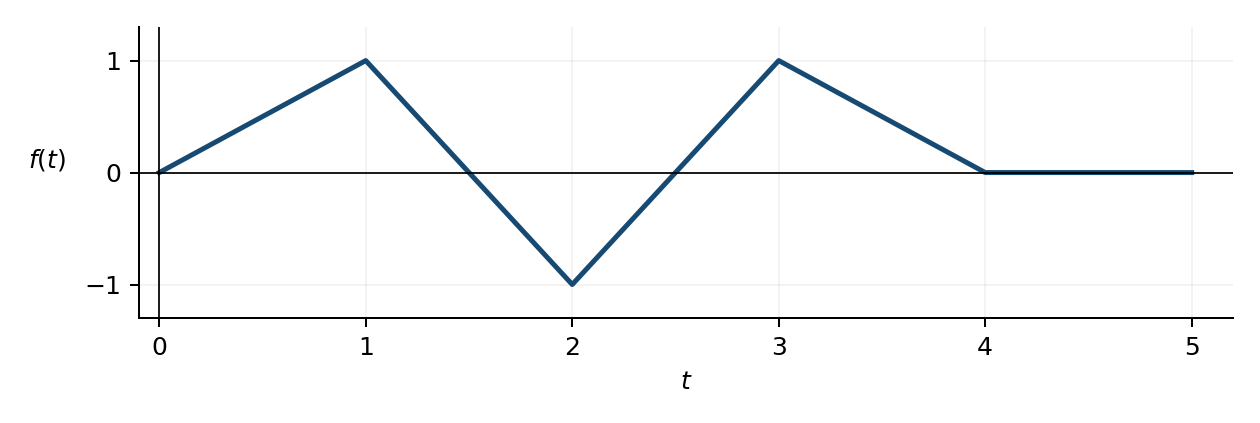
\includegraphics[width=.9\linewidth]{assets/M2-E0216-answer-graph.png}\end{center}

\noindent\textbf{(b)} $F(s)=(1-3e^{-s}+4e^{-2s}-3e^{-3s}+e^{-4s})/s^2$.

\noindent\textbf{(c)} Sea $R(t)=t-\sin t$ y $(c_0,c_1,c_2,c_3,c_4)=(1,-3,4,-3,1)$. Entonces
\[y(t)=\sin t+\sum_{j=0}^4c_jH(t-j)R(t-j).\]
